\input{_actp.latex}

% --- Titre et classe
\def\Titre{Suites numériques}
\def\Classe{1STMG}

% ---
\begin{document}
\MonTitre{Activité : \Titre}
\vspace*{0.7cm}
\section{Activité 1 : Listes de nombres à prolonger}
On donne les quatres listes de nombre suivantes :
\begin{center}$A:1;3;5;7;9\qquad B:1;3;9;27;81\qquad C:0;1;4;9;16;25\qquad D:3;6;11;18;27$\end{center}
\begin{enumerate}
	\item Indiquer comment chacunes est construite.
	\item Donner les deux nombres suivants de chaque liste.
	\item Pour quelles listes est-il possible de trouver le $20$\up{ème} nombre de la liste sans calculer tous ceux qui le précèdent ?
\end{enumerate}
\vspace*{0.7cm}
\section{Activité 2 : Une situation discrète}
Votre cinéma propose un tarif de $6$\euro~la séance pour les moins de 26 ans.

Ainsi, le coût total pour $3$ séances est de : $6\times 3=18$\euro~et, pour $5$ séances, $6\times 5=30$\euro.

Plus généralement, le coût total en \euro~, pour $x$ séances de cinéma, est $6\times x$.


\begin{enumerate}
	\item Tracer dans un repère la représentation de la fonction $f(x)=6x$
	\item \begin{enumerate}
		      \item Déterminer graphiquement la valeur de $x$ lorsque $f(x)=24$
		      \item Compléter : "Le coût total pour ...... séances est de ...... \euro"
	      \end{enumerate}
	\item Reprendre la question 2. pour $f(x)=15$.\par La phrase à compléter a-t-elle un sens dans ce cas ? pourquoi ?
\end{enumerate}

Nous venons d'étudier une situation où la variable $x$ pour la fonction $f$ définie par $f(x)=6x$ ne peut prendre que des valeurs entières : $1 ; 2 ; 3; ...$

Dans ce cas, en mathématiques, on a l'habitude de remplacer la lettre $f$ par $u$ et la variable $x$ par $n$.

Dans cet exemple, $u(n)=6n$.

En particulier $u(0)=0~,~u(1)=6~,~u(2)=12~,...$ et la représentation graphique de $u$ est constituée des seuls points d'abscisse \textit{entière} obtenus à la question 1.

\begin{enumerate}[resume]
	\item Représenter ces points par une croix.
\end{enumerate}
\vspace*{0.7cm}
\section{Activité 3 : Triangle de Sierpiński}
Ce triangle est obtenu en répétant l'algorithme suivant à partir d'un triangle équilatéral :
\begin{itemize}[label=$\bullet$]
	\item Pour chaque triangle rouge, tracer les segments joignants les milieux des cotés, de façon à obtenir 4 triangles.
	\item Retirer le triangle central.
\end{itemize}
\begin{center}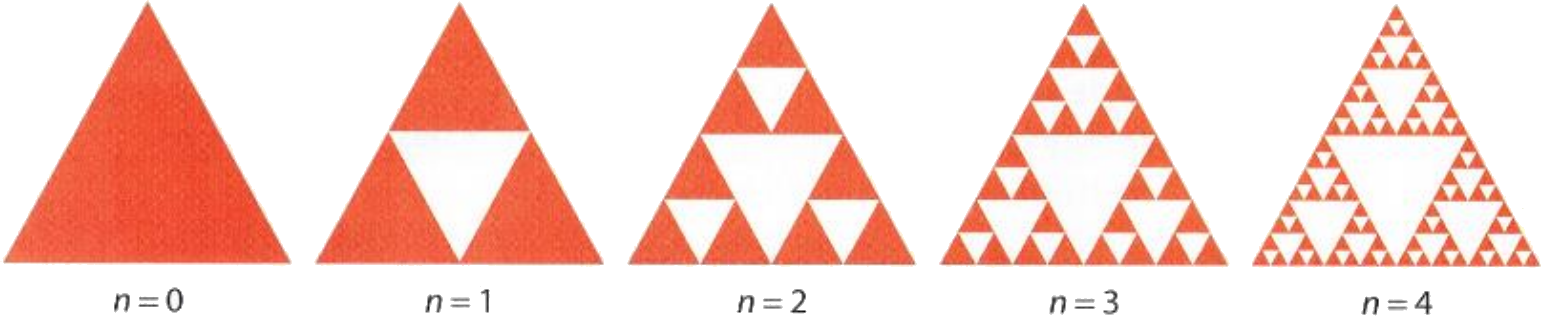
\includegraphics[width=18cm]{triangles.png}\end{center}
On part d'un triangle de 10cm de coté et on note $n$ le nombre d'itération de l'algorithme, c'est à dire le nombre de fois que l'algorithme est utilisé.

\begin{enumerate}
	\item Chaque fois que l'on passe d'une figure à la suivante, c'est-à-dire que l'on utilise une fois de plus l'algorithme, indiquer sans explication par une courte phrase ce que devient ...
	      \begin{enumerate}
		      \item ... le nombre de triangles rouges
		      \item ... la longueur d'un côté d'un triangle rouge
		      \item ... l'aire d'un triangle rouge
	      \end{enumerate}
\end{enumerate}
\end{document}
